\section{Busca em tabela de dispersão} \label{cap:3:section:hash}

\subsection{Introdução}

O algoritmo de busca em tabela de dispersão, funciona de modo que, através da função
hash, eu ache um item mapeado para a chave $x$, com isso, se o item for nulo, o elemento
$x$ não está presente, se não for nulo, a lista encadeada é transcorrida até acharmos ou não
o elemento $x$.

\subsection{Implementação}

A implementação do algoritmo de busca em tabela de dispersão consiste em achar o item mapeado para
$x$ usando a função $hash(x)$ e após isso, se o valor da posição não for nulo, transcorrer a lista
até achar ou não o elemento $x$.

\begin{lstlisting}[style=CStyle]
int searchHashTable(HashTable * hashTable, int key) 
{
    int hashIndex = hashFunction(key);
    HashItem * temp = hashTable->table[hashIndex];

    while (temp != NULL) {
        if (temp->key == key) {
            return temp->value;
        }
        temp = temp->next;
    }

    return -1;
}
\end{lstlisting}
                

Seu tempo de execução é na ordem da equação \ref{cap:3:eq:hash}.

\begin{equation} \label{cap:3:eq:bTree}
    T(n) = \Theta(1)
\end{equation}

\subsection{Resultados}

Para a implementação, foi obtido o gráfico \ref{cap:3:graph:hash}:

\begin{figure}[h]
    \centering
    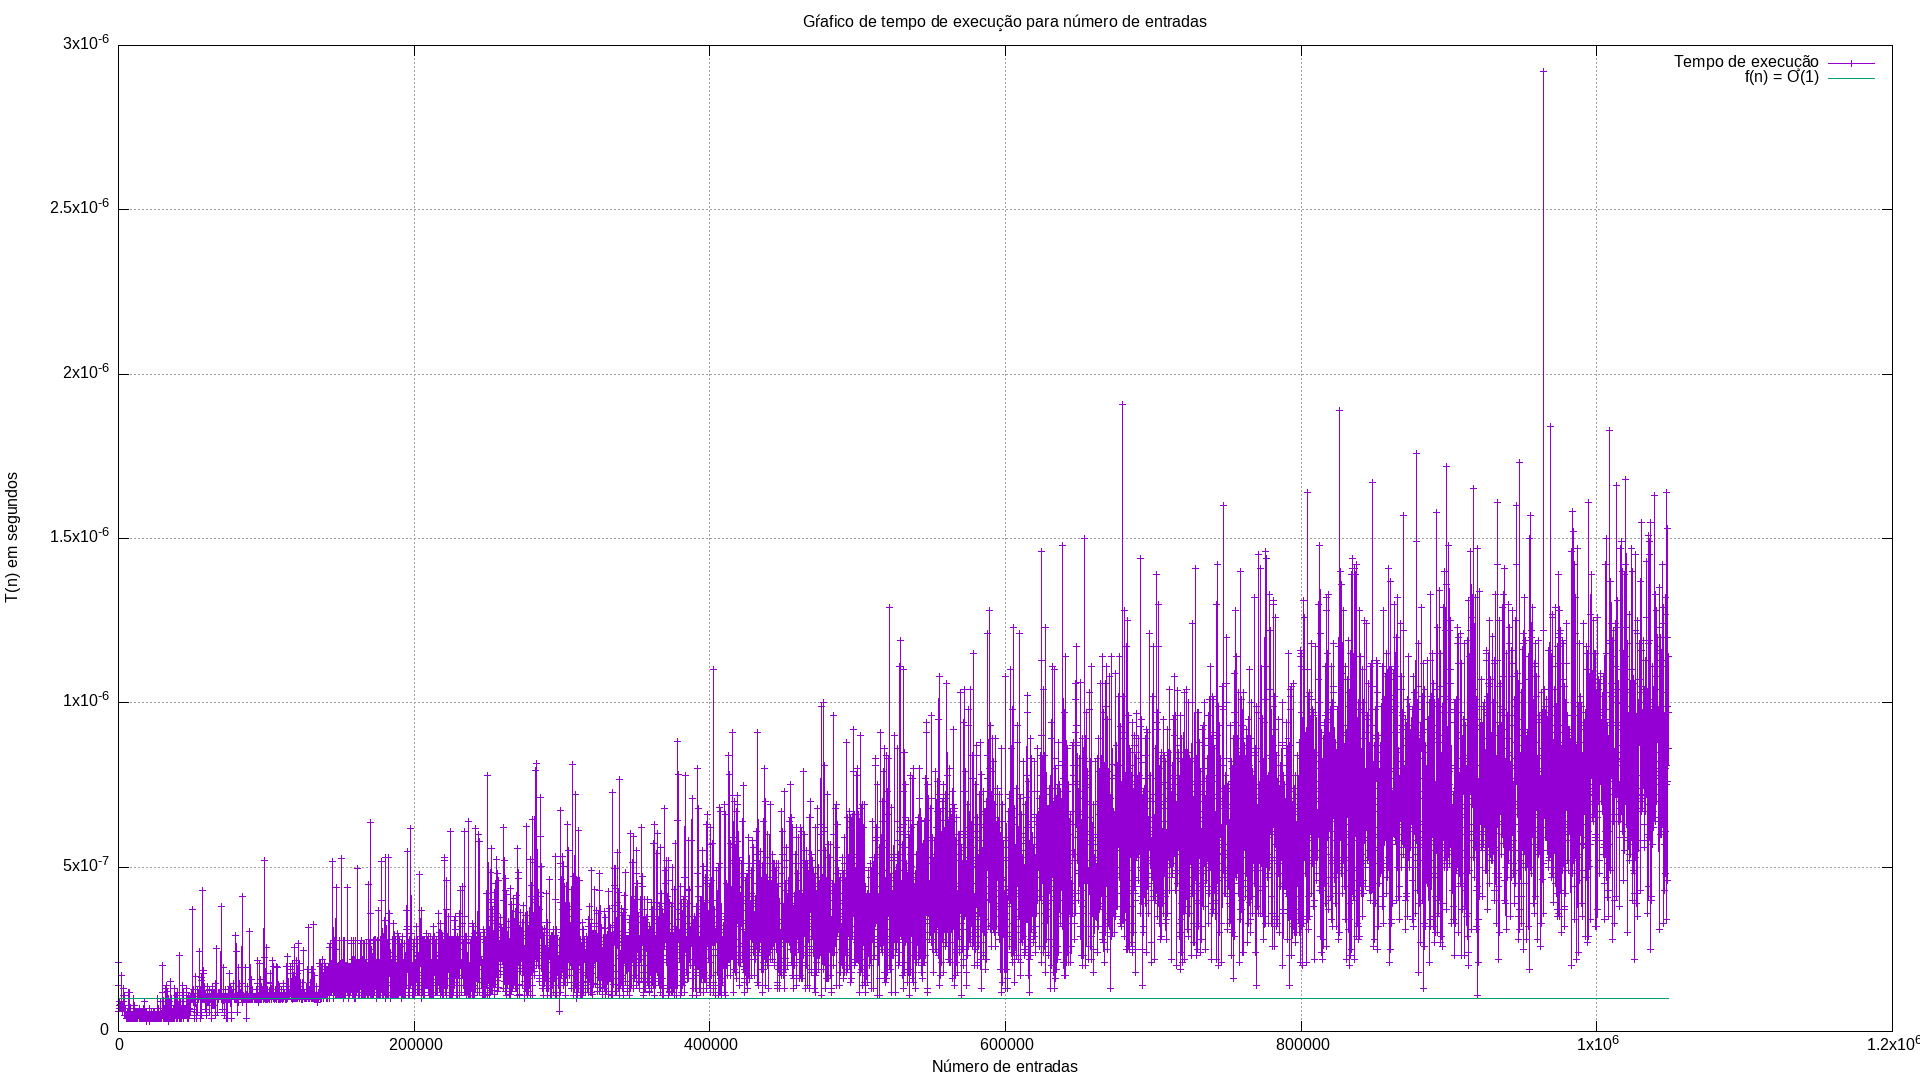
\includegraphics[width=\textwidth]{image/graphics/hash.png}
    \caption{Gráfico com tempo de execução do algoritmo de busca em tabela de dispersão}
    \label{cap:3:graph:hash}
\end{figure}

O gráfico obtido indica que:
